% -----------------------------*- LaTeX -*------------------------------
\documentclass[12pt]{report}
\usepackage{scribe_hgen486}
\def \baselinestretch{1.2}
\def\ni{\noindent}
\def\Be{\text{Be}}

\usepackage{amsmath,url,enumerate,graphicx}

\usepackage{chngcntr}
\counterwithout{table}{section}
\begin{document}

\scribe{Alan Hutchison}		% required
\lecturenumber{5}			% required, must be a number
\lecturedate{January 19}		% required, omit year
\lecturer{Matthew Stephens} 

\maketitle

% please leave this comment 
\framebox[.95\textwidth]{\parbox{.93\textwidth}{ {{\bf Note:}} These
lecture notes are still rough, and have only have been mildly
proofread.  }}
\vspace*{.1in}


% feel free to delete content below this line 
% ----------------------------------------------------------------------




\section{Introduction to Bayesian Inference}

\emph{See github.com/stephens999/stat302 for further notes by M. Stephens on Bayesian Inference (Lects. 1-4)}

From last class:\
Posterior Odds = Prior Odds * Likelihood Ratio (aka Bayes Factor)

\[
\frac{Pr(M_1|x)}{Pr(M_0|x)} = \frac{P(M_1)}{P(M_0)} * \frac{P(x|M_1}{P(x|M_0)}
\]

This is the two model $M_1$ vs. $M_0$ case. We saw two examples of this in the previous lecture, regarding 1) Identifying Elephant Tusks and 2) Protein measurements in the blood. In these cases we were using likelihood ratios (LRs) for imagining a population that we're screening to tell us the conditional probability of a state (elephant type of tusk / disease state of patient) given data.\\

What if we only have 1 tusk and a LR of 1.8? We can think of the LR as a measure of the uncertainty of event (tusk is Savannah, tusk is Forest) based on everything we know. Instead of thinking in terms of a `measure of frequency' we can think in terms of a `measure of uncertainty'.\\

\begin{enumerate}
\item ``50\% chance of snow tomorrow'' This is simplest understood as the uncertainty of snow, not as a prediction of a hypothetical population of days.
\item The answer to ``Did it snow in Denver?'' can be expressed as an uncertainty, even though the event `snowed in Denver' is not a random variable.
\end{enumerate}

One way of thinking about uncertainty is by ``comparing an event to a standard'', such as a flip of a (fair) coin or a roll of a (fair) dice. It is not unreasonable to start with these standards (usually uniformly distributed probabilities). Heuristically, if one's prior odds are off by a factor of 10, then it starts to be more problematic.

\section{Comparison of more than two models}

Now, we will look at $k$ different models instead of 2 models, as we have done previously.\\

In the elephant case, for example, instead of thinking of just Forest vs. Savannah elephants, we could think about further subdividing these categories by genetic differences amongst the different cardinal directions (N E S W). \\

Let's refer to the different models as $Z_i \in \{1,2,...,k\}$, the likelihood of data $P(x_i|Z_i=k)$ as $L_{ik}$ and the prior probability $P(Z_i=k)$ as $\Pi_k$. We are using subscript $i$ to denote a series of tusks, but we could just as easily drop the $i's$.\\

Using the Law of Total Probability (LTP), we can write

\[
P(x_i) = \sum_{k'} P(x_i,Z_i=k') = \sum_{k'} P(x_i | Z_i=k') P(Z_i = k') = \sum_{k'} L_{ik'} \Pi_{k'}
\]
\[
P(Z_i=k|x_i) = \frac{P(x_i|Z_i=k)P(Z_i=k)}{P(x_i)} = \frac{L_{ik}\Pi_k}{\sum_{k'} L_{ik'} \Pi_{k'}}.
\]

Note that the denominator is simply the sum over $k$ of all possible numerators. We use the symbol $k'$ to denote the same set of states $k$, only for the sum across all $k$ of them. This means we can simply compute $L_{ik}\Pi_k$ for each $k$, then divide by the sum of them at the end. If all $k$ models are equally likely, then we end up just normalizing by the sum of the likelihoods.\\

Instead of using equalities, we can use proportions to avoid thinking about the normalizing factor. We can think about this as informing our posterior uncertainty by what we learn from the data (the likelihood) with what we knew or believed beforehand (the prior).
\[
Posterior \propto Likelihood * Prior
\]

Remember that the likelihoods themselves don't really matter, it's the ratios that give you information about the different models. In ratios the normalizing constant ends up canceling out altogether.

\section{Continuum of models case: Parametric model}
\subsection{Estimating an allele frequency}

As previously, sample 100 alleles, see 40 of type `1' and 60 of type `0'. $D$: Data. $M_q$: ``freq. of allele `1' is q''\\

Originally we used,
\[
L(q) = q^{40} (1-q)^{60}
\]

Maximizing this provides a Maximum Likelihood Estimate (MLE) point estimate for $q$, but we may be interested incorporating prior information or belief for $q$. We can compute the posterior distribution of $q$ using Bayes Theorem. Let our prior distribution on $q$ be $P(q)$.

\[
P(q|D) \propto q^{40} (1-q)^{60} * p(q)
\]
Assuming that all values of $q$ are equally probable $P(q)=1$

\[
P(q|D) \propto q^{40} (1-q)^{60}
\]
 now we need to normalize by $\int q'^{40}(1-q')^{60} dq'$. This normalization step can be a complicated integral, and there are some shortcuts that can be used here. Instead of solving out the integral, it is easier if we can recognize it as a standard distribution whose behavior we know.

 Since we are used the assumption that $P(q)=1$, i.e. all values of $q$ are equally probable, we can also write this uniform distribution as a Beta distribution of $q$, $Be(q;\alpha,\beta)=q^{1-\alpha} (1-q)^{1-\beta}$ with parameters $\alpha=1$ and $\beta=1$, $P(q) = Be(q;1,1) = q^0 (1-q)^0 = 1$.

\[
P(q|D) \propto q^{40} (1-q)^{60} * p(q) =  q^{40} (1-q)^{60} q^0 (1-q)^0 = q^{40} (1-q)^{60}
\]

Rewritten as a Beta distribution, we have


\[
P(q|D) \propto q^{40} (1-q)^{60} = q^{\alpha -1 = 40} (1-q)^{\beta -1 = 60} = Be(q;\alpha,\beta) = Be(q;41,61)
\]

Having an expression proportional to the posterior distribution $P(q|D)$, we have the means for summarizing $q$ as either a point estimate or as an interval. For point estimates, common choices include the \emph{posterior mean}, \emph{posterior median}, and \emph{posterior mode}. For an interval estimate, \emph{posterior quantiles} allow us to describe the spread of likely values of $q$. Giving the 2.5\% quantile and 97.5\% quantile provides the interval for which there is a 95\% probability that $q$ lies in it.


There are two takeaways from this section

\begin{enumerate}
\item For computing the posterior distribution in the continuous case, we use the same procedure as the the discrete case but we have the trick of using conjugate prior distributions to make the math simpler.
\item Once we have the posterior distribution, we can summarize it with both point estimates and interval estimates.
\end{enumerate}

\subsection{Conjugacy}

 For many types of likelihood functions there are corresponding prior \emph{conjugate} distributions such that when the two are multiplied together the resulting distribution is also in the same family of conjugate distributions. More formally, \emph{conjugacy means that the posterior distribution comes from the same family as the prior distribution}. These priors may not be realistic interpretations of the underlying mechanism of the prior distribution, but they are powerful and useful. For the Beta distributions in particular, any distribution with support of [0,1] can be approximated as a mixture of Beta distributions.

A question in class asked if there were any properties of likelihood functions that would indicate whether a conjugate prior distribution exists. The short answer is no, though it has been proven that exponential likelihood families have conjugate priors. Many common distributions have been identified as having conjugate priors, and they are summarized in Table \ref{tab:test}.

\begin{table}
\begin{center}
\begin{tabular}{|c|c|}\hline
Observed Likelihood Function & Conjugate Prior \\ \hline \hline
Binomial & Beta \\ \hline
Multinomial & Dirichlet \\ \hline
Mean of Normal & Normal \\ \hline
Variance of Normal & Inverse Normal \\ \hline
Mean of Poisson & Gamma \\ \hline
\end{tabular}
\caption{Observed Likelihood Functions and their Conjugate Priors}
\label{tab:test}
\end{center}
\end{table}

Let's return to the above example. Instead of assuming the uniform prior distribution $P(q) = Be(q;1,1)$, let's leave it as a general Beta distribution.

\[
P(q|D) \propto q^{40} (1-q)^{60} * p(q) =  q^{40} (1-q)^{60} q^{\alpha-1} (1-q)^{\beta-1} = q^{40+\alpha-1} (1-q)^{60+\beta-1} = Be(q;40+\alpha,60+\beta)
\]

Here we can see exactly how the choice of the prior distribution parameters $\alpha$ and $\beta$ can include the resulting posterior distribution. Figure \ref{fig:2015-01-19_beta} shows the Beta distribution for a variety of $\alpha,\beta$ combinations.

\begin{figure}
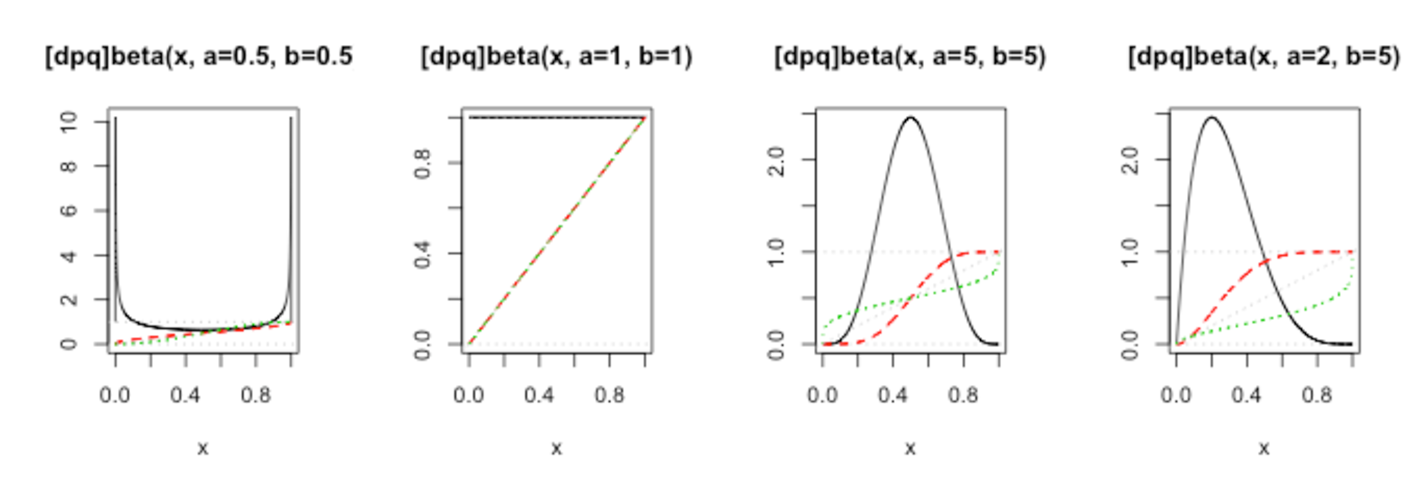
\includegraphics[width=\textwidth]{Betas.pdf}
\label{fig:2015-01-19_beta}
\caption{Beta distributions for different $\alpha$ and $\beta$ values. Black refers to the density, red to the distribution function, and green the quantile function.}
\end{figure}

 Given that it is reasonable to assume that the prior distribution of allele frequencies in population genetics is U-shaped, we can use a prior distribution of $Be(q;0.5,0.5)$.

 \[
P(q|D) \propto  q^{40} (1-q)^{60} q^{1/2-1} (1-q)^{1/2-1} = q^{40-1/2} (1-q)^{60-1/2} = Be(q;40.5,60.5)
\]
As you can see, this slightly changes our posterior distribution with a uniform prior, from $Be(q;41,61)$ to $Be(q;40.5,60.5)$


More generally, we can think of the observed alleles in our sample as $n_1$ of type ``1'' and $n_0$ of type ``0''. This means our posterior distribution will be

\[
P(q|D) \sim\  Be(q;n_1+\alpha,n_0+\beta)
\]

and the resulting posterior mean estimate for $q$ would be

\[
E[P(q|D)] = \frac{n_1+\alpha}{n_0+n_1+\alpha+\beta}
\]

Using a Maximum Likelihood Estimate (MLE) approach instead, our result would be independent of the prior distribution

\[
E[L(q|D)] = \frac{n_1}{n_0+n_1}
\]

Likewise, estimating $q$ solely off the prior distribution would be independent of observed data $n_0$ or $n_1$.

\[
E[Be(q;\alpha,\beta)] = \frac{\alpha}{\alpha+\beta}
\]

What this comparison of point estimates of $q$ shows is that the posterior mean of $q$ is a combination or tradeoff or compromise of the MLE estimate and the prior estimate: the results is `weighted' by the evidence presented by $n_0$ and $n_1$, but is balanced against the prior information or uncertainty about the population encoded in $\alpha$ and $\beta$. If $\alpha$ and $\beta$ are big relative to $n_0$ and $n_1$, then the posterior mean will be close to the prior mean. If $n_0$ and $n_1$ are big relative to $\alpha$ and $\beta$, then the posterior mean will be close to the MLE. ``In sufficient quantities, data can overwhelm belief.''

Note: in some situations, $\alpha$ and $\beta$ can be thought of as pseudo-counts. This can be useful in a situation where you want a prior that strongly discounts the possibility of an event but you don't want to make it zero. In that case, you could use a prior of $Be(1,100)$ to indicate the prior belief that it is extremely unlikely and then let the data determine whether the posterior probability of the event increases.

\subsection{Example: Estimating Normal Mean}

1 observation: data $X \sim\ N(\theta,\sigma^2)$

assuming $\sigma^2$ is known (e.g. measurement error).

Prior on $\theta$, $\theta \sim\ N(\mu_0,\sigma_0^2)$. We use the subscript `0' to denote that these are prior parameters.

\[
P(\theta|X=x) \propto\ prior * likelihood
\]
\[
P(\theta|X=x) \propto\ \exp{[\frac{-(\theta - \mu_0)^2}{2 \sigma_0^2}]} \exp{[\frac{-(x - \theta)^2}{2 \sigma^2}]}
\]


\[
P(\theta|X=x) \propto\ \exp{[\theta^2 [-\frac{1}{2\sigma_0^2}+\frac{1}{2\sigma^2}] + \theta[\frac{\mu_0}{\sigma_0^2}+\frac{x}{\sigma^2}]]}
\]

Given we are solving for the normal mean using a normal conjugate prior, we know our posterior distribution is going to have the form
\[
P(\theta|X=x) \propto\ N(\mu_1,\sigma_1^2) = \exp{[\frac{-(\theta - \mu_1)^2}{2 \sigma_1^2}]}
\]

which can be re-written without the constants as

\[
P(\theta|X=x) \propto\  \exp{[\theta^2\frac{-1}{2 \sigma_1^2}+\theta \frac{-\mu_1^2}{2 \sigma_1^2}]}
\]




Comparing this with the above equation, we can determine that

\[
\frac{1}{\sigma_1^2} = \frac{1}{\sigma_0^2} + \frac{1}{\sigma^2}
\]
The inverse of the variance $\frac{1}{\sigma^2}$ is referred to as the precision, which is mathematically sometimes more tractable. This equation means that our posterior precision is the sum of our prior precision and our precision from our data. Our precision gets bigger, and our variance gets smaller.

\[
\frac{\mu}{\sigma_1^2} = \frac{\mu_0}{\sigma_0^2} + \frac{x}{\sigma^2}
\]

This means that the product of our posterior mean and our posterior precision is the sum of the product of our prior mean and prior precision with product of our observed $x$ and observed precision.


\end{document}


